\documentclass[12pt,compress]{beamer}
\usepackage{amsmath}
\usepackage{url}
\usepackage{ucs}
\usepackage[utf8x]{inputenc}
\usepackage[ngerman]{babel}
\usepackage{bbm}
\usepackage{ulem}
\usepackage{multicol}
\usepackage{setspace}
\usepackage{color}
\usepackage{hyperref}

\usetheme{Boadilla}
\setbeamertemplate{footline}%{infolines theme}

\usecolortheme{lily}
\useinnertheme{circles}
\setbeamercovered{transparent}
\beamertemplatenavigationsymbolsempty

\definecolor{darkgreen}{rgb}{0,0.5,0}

\hypersetup{
    bookmarks=true,
    unicode=true,
    pdftoolbar=true,
    pdfmenubar=true,
    pdffitwindow=false,
    pdfstartview={FitH},
    pdftitle={Logistische Abbildung},
    pdfauthor={Michael Hartmann},
    pdfsubject={Vortrag über die logistische Abbildung},
    pdfcreator={vim},
    pdfproducer={pdflatex},
    pdfkeywords={chaos} {logitische Abbildung},
    pdfnewwindow=true,
    colorlinks=true,
    linkcolor=black,
    citecolor=green,
    filecolor=magenta,
    urlcolor=darkgreen
}



\title{Chaos II: Differentialgleichungen}
\institute{Kaffeeseminar}
\author{Michael Hartmann}
\date{6. November 2015}


\begin{document}

\begin{frame}
    \titlepage
\end{frame}

\frame {
    \tableofcontents
}

\section{Lineare Differentialgleichungen}
\subsection{Lösung}
\frame {
    \frametitle{Differentialgleichungen}

    Wir betrachten lineare, homogene Differentialgleichungen
    \begin{equation}
    \nonumber
    \frac{\mathrm{d}}{\mathrm{d}t} \vec x = \mathcal{L} \vec x,
    \end{equation}
    wobei $\mathcal{L}$ (nicht singuläre) $n\times n$ Matrix mit konstanten Koeffizienten.
    
    \pause
    \vfill

    Lösung:
    \begin{equation}
    \nonumber
    \vec x(t) = e^{\mathcal{L}(t-t_0)} \vec x(t_0)
    \end{equation}

    \pause
    \vfill

    Verhalten der Lösung wird durch die Eigenwerte von $\mathcal{L}$ bestimmt!
}

\subsection{Beispiele in 2D}
\frame {
    \frametitle{Beispiele in 2D}

    \begin{center}
    \only<1>
    {
    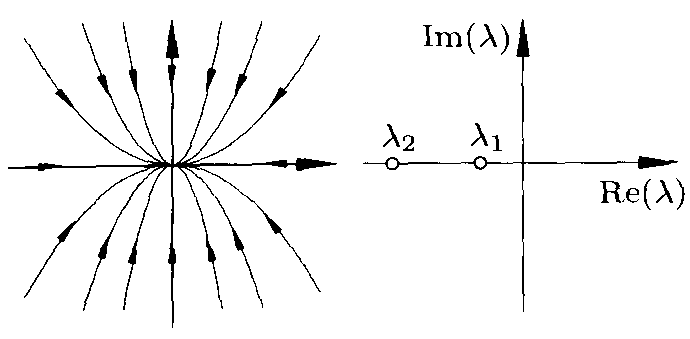
\includegraphics[scale=0.5]{01_stable_node.png}

    stable node
    }
    \only<2>
    {
    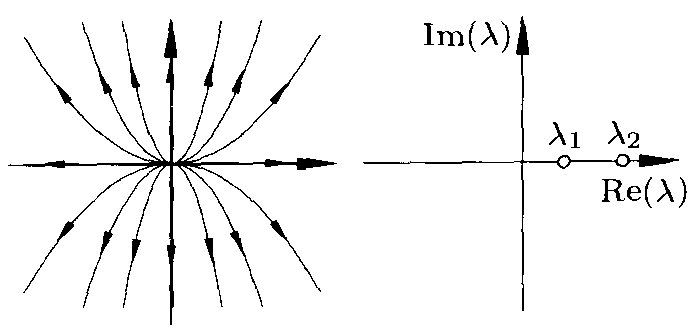
\includegraphics[scale=0.5]{02_unstable_node.png}

    unstable node
    }
    \only<3>
    {
    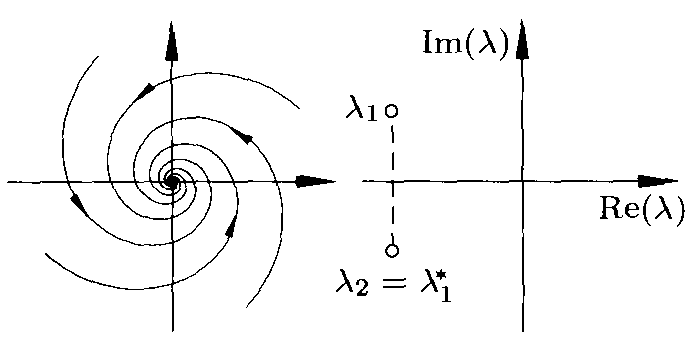
\includegraphics[scale=0.5]{03_stable_focus.png}

    stable focus
    }
    \only<4>
    {
    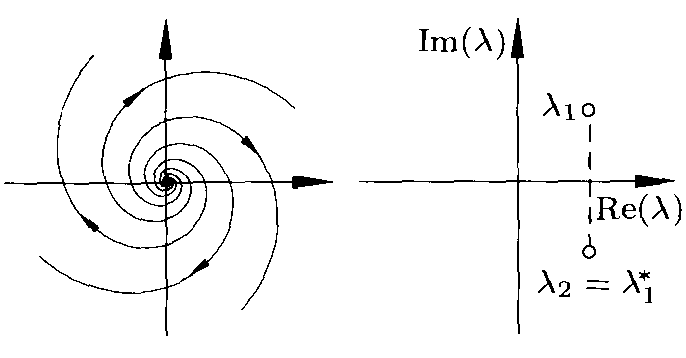
\includegraphics[scale=0.5]{04_unstable_focus.png}

    unstable focus
    }
    \only<5>
    {
    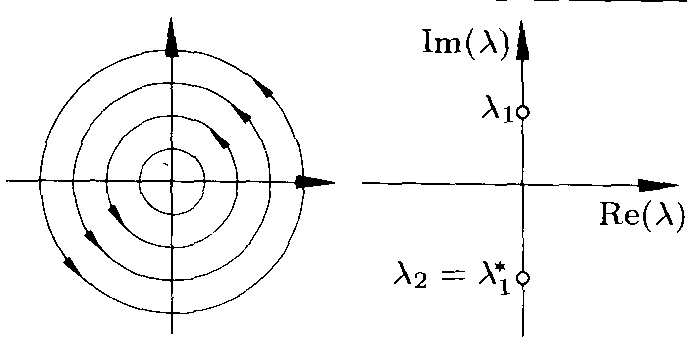
\includegraphics[scale=0.5]{05_center_point.png}

    center point
    }
    \only<6>
    {
    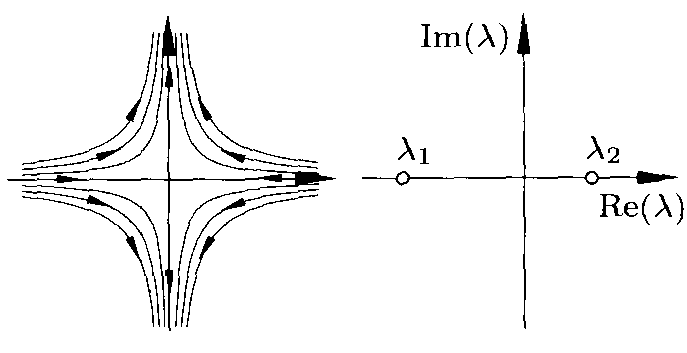
\includegraphics[scale=0.5]{06_saddle_point.png}

    saddle point
    }

    \only<7>
    {
    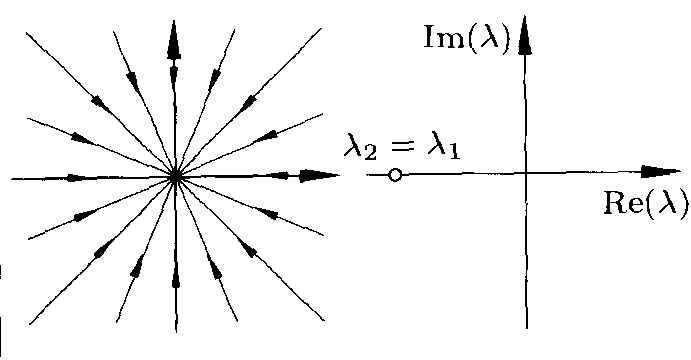
\includegraphics[scale=0.5]{07_star.png}

    star ($\mathcal{L}$ diagonalisierbar)
    }
    \only<8>
    {
    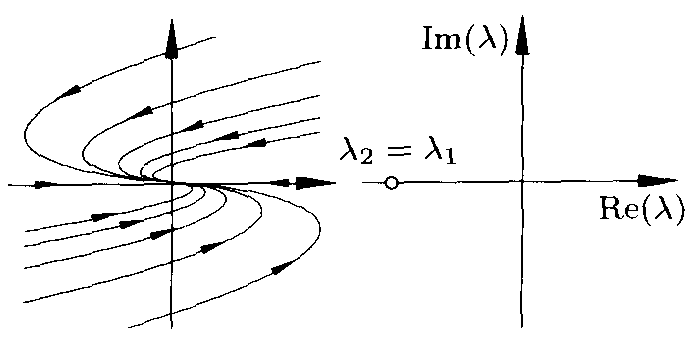
\includegraphics[scale=0.5]{08_stable_node.png}

    stable node ($\mathcal{L}$ nicht diagonalisierbar)
    }
    \only<9>
    {
    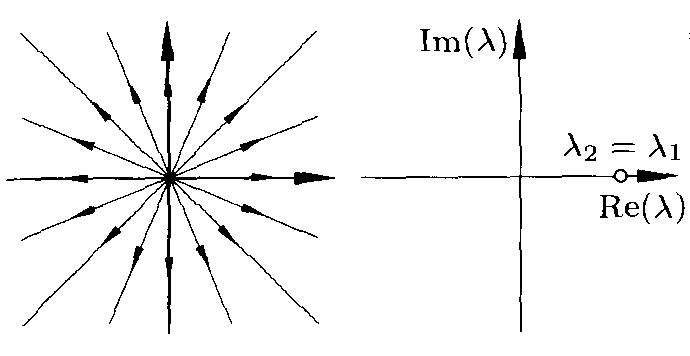
\includegraphics[scale=0.5]{09_unstable_star.png}

    unstable star ($\mathcal{L}$ diagonalisierbar)
    }
    \only<10>
    {
    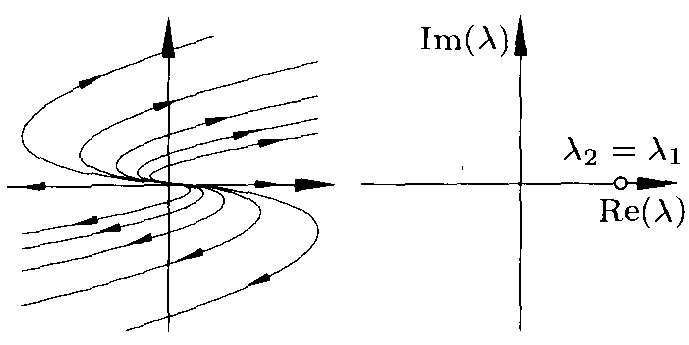
\includegraphics[scale=0.5]{10_unstable_node.png}

    unstable node ($\mathcal{L}$ nicht diagonalisierbar)
    }
    \end{center}

    \vfill
    \noindent\rule{8cm}{0.4pt}

    An Exploration of Chaos, Argyris, Faust, Haase
}

\subsection{Beispiel: gedämpfter harmonischer Oszillator}
\frame {
    \frametitle{Beispiel: gedämpfter harmonischer Oszillator}

    \only<1,2,3>
    {
    Harmonischer Oszillator mit linearer Dämpfung:
    \begin{equation}
    \nonumber
    \ddot x + 2\gamma \dot x + \omega_0^2 x = 0
    \end{equation}

    \pause
    \vfill

    Als System 1. Ordnung:
    \begin{equation}
    \nonumber
    \left(\begin{array}{c} \dot x \\ \dot v \end{array}\right) = \left(\begin{array}{cc} 0 & 1 \\ -\omega_0^2 & -2\gamma \end{array}\right) \left(\begin{array}{c} x \\ v \end{array}\right)
    \end{equation}

    \pause
    \vfill
    Eigenwerte:
    \begin{equation}
    \nonumber
    \lambda^2 + 2\gamma\lambda + \omega_0^2 = 0 \qquad \Rightarrow \qquad \lambda_{1,2} = -\gamma \pm \sqrt{\gamma^2-\omega_0^2}
    \end{equation}
    }

    \only<4>
    {
    $\gamma = 0$: $\lambda_{1,2} = \pm i\omega_0$

    \begin{center}
    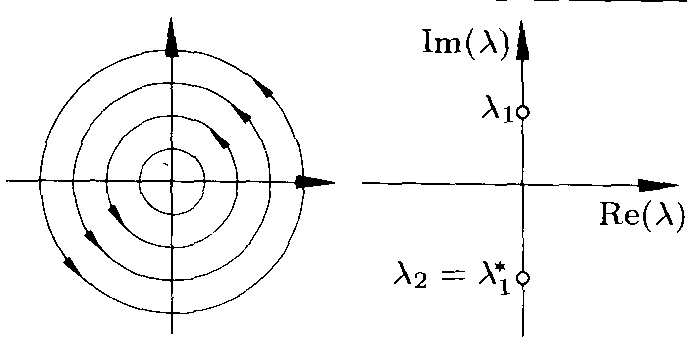
\includegraphics[scale=0.5]{05_center_point.png}
    \end{center}
    }

    \only<5>
    {
    $0 < \gamma < \omega_0$: $\lambda_{1,2} = -\gamma \pm i \sqrt{\omega_0^2-\gamma^2}$

    \begin{center}
    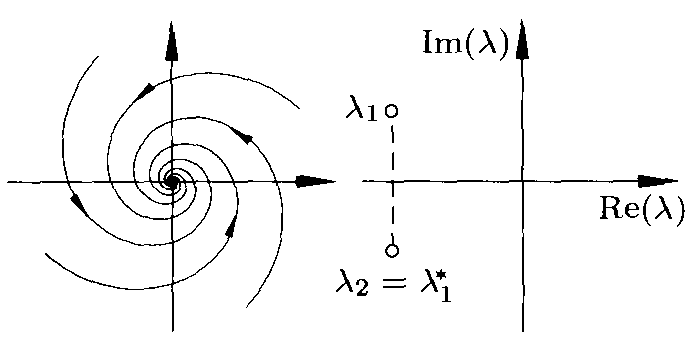
\includegraphics[scale=0.5]{03_stable_focus.png}
    \end{center}
    }

    \only<6>
    {
    $\gamma = \omega_0$: $\lambda_{1,2} = -\gamma$ (Matrix {\it nicht} diagonalisierbar)

    \begin{center}
    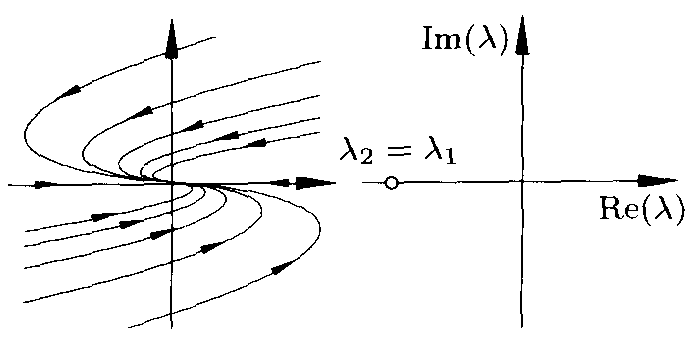
\includegraphics[scale=0.5]{08_stable_node.png}
    \end{center}
    }

    \only<7>
    {
    $\gamma > \omega_0$: $\lambda_{1,2} = -\gamma \pm \sqrt{\gamma^2-\omega_0^2}$

    \begin{center}
    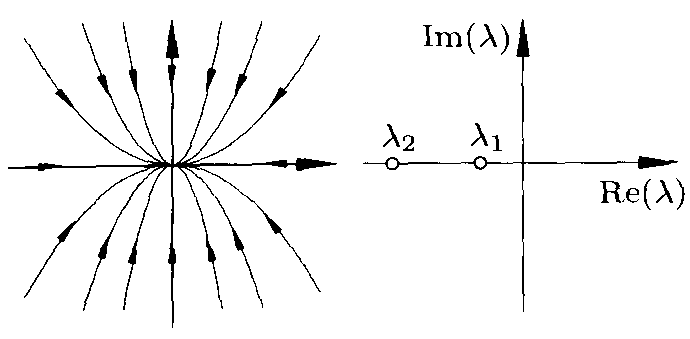
\includegraphics[scale=0.5]{01_stable_node.png}
    \end{center}
    }

    \only<4->
    {
    \vfill
    \noindent\rule{8cm}{0.4pt}

    An Exploration of Chaos, Argyris, Faust, Haase
    }
}

\section{autonome, nicht-lineare Differentialgleichungen}
\subsection{Stationäre Punkte und Stabilität}
\frame {
    \frametitle{autonome, nicht-lineare Differentialgleichungen}

    Wir interessieren uns für allgemeine DGl (autonom):
    \begin{equation}
    \nonumber
    \dot{\vec{x}} = \vec{f}(\vec x)
    \end{equation}
    
    \pause
    \vfill

    Stationäre Punkte:
    \begin{equation}
    \nonumber
    \vec{f}(\vec x_s) = 0
    \end{equation}

    \pause
    \vfill

    Stabilität: um stationären Punkt entwickeln:
    \begin{equation}
    \nonumber
    \frac{\mathrm{d}}{\mathrm{d}t} \left(\vec{x}_s+\delta\vec{x}\right) \approx J_f\left(\vec x_s\right)\delta\vec x
    \end{equation}
}

\subsection{Beispiel: Fadenpendel}
\frame {
    \frametitle{Beispiel: Fadenpendel}

    \only<1,2,3> {
    Differentialgleichung:
    \begin{equation}
    \nonumber
    \ddot x + \omega_0^2 \sin x = 0
    \end{equation}

    \pause
    \vfill

    Als System 1. Ordnung:
    \begin{equation}
    \nonumber
    \left(\begin{array}{c} \dot x \\ \dot v \end{array}\right) = \vec{f}(x,v) = \left(\begin{array}{c} v \\ -\omega_0^2 \sin x\end{array}\right)
    \end{equation}

    \pause
    \vfill

    Stationäre Punkte:
    \begin{itemize}
    \item $(x^s_1, v^s_1) = (0, 0)$
    \item $(x^s_2, v^s_2) = (\pi, 0)$
    \end{itemize}
    }

    \only<4,5>
    {
        $(x^s_1, v^s_1) = (0, 0)$:
        \begin{itemize}
        \item Linearisieren:
        \begin{equation}
        \nonumber
        \vec{f}\left(\begin{array}{c} x^s_1+\delta x \\ v^s_1+\delta v\end{array}\right) \approx \left(\begin{array}{cc} 0 & 1 \\ -\omega_0^2 & 0 \end{array}\right) \left(\begin{array}{c} \delta x \\ \delta v \end{array}\right)
        \end{equation}
        \item Eigenwerte: $\lambda_{1,2} = \pm i\omega_0^2$
        \item[$\Rightarrow$] stabiler stationärer Punkt, Oszillationen
        \end{itemize}

        \vfill
        \pause

        \only<5>
        {
        \begin{center}
        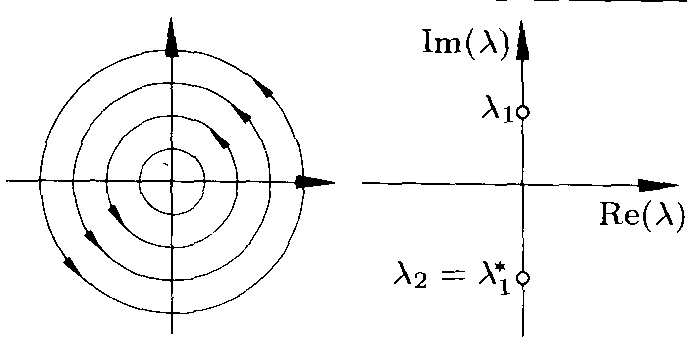
\includegraphics[scale=0.25]{05_center_point.png}
        \end{center}
        }
    }

    \only<6,7>
    {
        $(x^s_2, v^s_2) = (0, \pi)$:
        \begin{itemize}
        \item 
        \begin{equation}
        \nonumber
        \vec{f}\left(\begin{array}{c} x^s_2+\delta x \\ v^s_2 + \delta v\end{array}\right) \approx \left(\begin{array}{cc} 0 & 1 \\ \omega_0^2 & 0 \end{array}\right) \left(\begin{array}{c} x \\ v \end{array}\right)
        \end{equation}
        \item Eigenwerte: $\lambda_{1,2} = \pm\omega_0^2$
        \item[$\Rightarrow$] instabiler stationärer Punkt
        \end{itemize}

        \vfill

        \only<7>
        {
        \begin{center}
        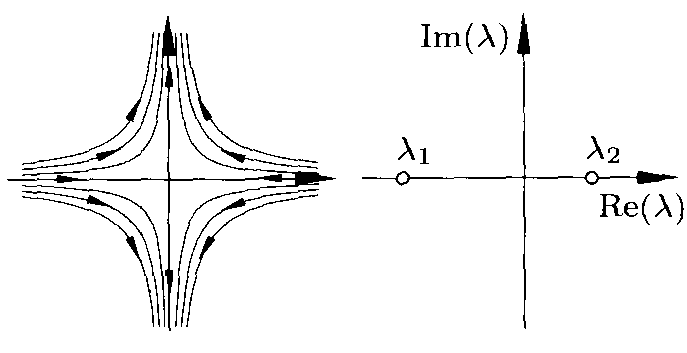
\includegraphics[scale=0.3]{06_saddle_point.png}
        \end{center}
        }
    }
}

\subsection{komplexeres Beispiel}
\frame {
    \frametitle{Weiteres Beispiel}

    Differentialgleichung:
    \begin{equation}
    \nonumber
    \left(\begin{array}{c} \dot\vartheta \\ \dot\varphi\end{array}\right) = \vec f(\vartheta,\varphi) =
    \left(\begin{array}{c}
    A\sin\varphi+C\cos\varphi\cos\vartheta \\
    A \frac{\cos\vartheta}{\sin\vartheta}\cos\varphi + B\cos\vartheta - C\frac{\sin\varphi}{\sin\vartheta}
    \end{array}\right)
    \end{equation}

    \pause
    \vfill

    Stationäre Punkte: $\vec f = 0$
    \begin{itemize}
    \item $\dot\vartheta = 0$:
    \begin{equation}
    \nonumber
    \cos\vartheta = -\frac{A}{C}\tan\varphi, \quad \sin\vartheta = \sqrt{1-\frac{A^2}{C^2}\tan^2\varphi}
    \end{equation}
    \item $\dot\varphi = 0$:
    \begin{equation}
    \nonumber
    \sin\varphi \left[ \left(\frac{A^2}{C^2}+1\right)\cos\varphi + \frac{AB}{C^2}\sqrt{1-\frac{A^2}{C^2}\tan^2\varphi} \right] = 0
    \end{equation}
    \end{itemize}
}

\frame {
    \frametitle{Stationäre Punkte}

    \only<1>
    {
    \begin{itemize}
    \item stationäre Punkte hängen nur von $A/C$ und $B/C$ ab
    \item $\sin\varphi=0$:
    \begin{itemize}
    \item $(\vartheta,\varphi) = (\pi/2, 0)$: stabil falls $C^2 > -A(A+B)$
    \item $(\vartheta,\varphi) = (\pi/2, \pi)$: instabil
    \end{itemize}
    \item falls $\varphi$ stabiler (instabiler) stationärer Punkt, dann auch $-\varphi$
    \item weitere stationäre Punkte für Lösungen von:
    \begin{equation}
    \nonumber
    \left(\frac{A^2}{C^2}+1\right)\cos\varphi + \frac{AB}{C}\sqrt{1-\frac{A^2}{C^2}\tan^2\varphi}, \quad\quad |\varphi| \le \arctan\left|\frac{C}{A}\right|
    \end{equation}
    \end{itemize}
    }

    \only<2>
    {
        \begin{center}
        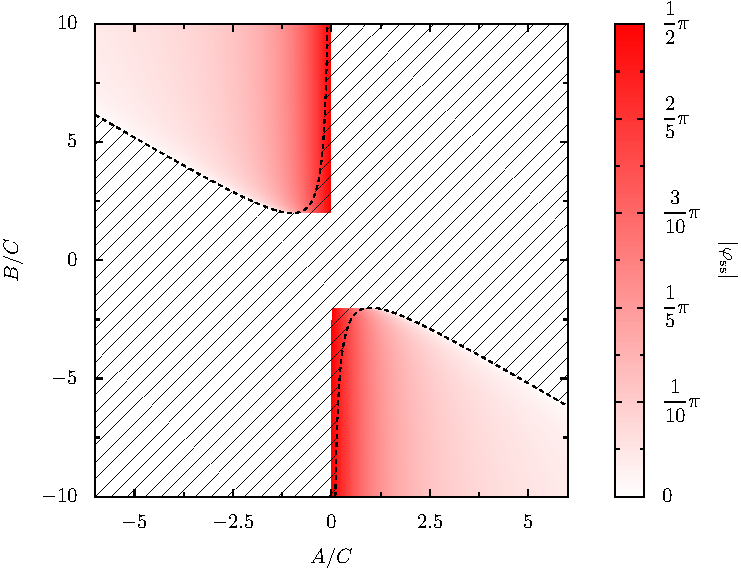
\includegraphics[scale=0.75]{nondriven.pdf}
        \end{center}
    }
}

\frame {
    \frametitle{Beispiel}

    $A/C=0.2$, $B/C=-2.5$:
    \begin{center}
    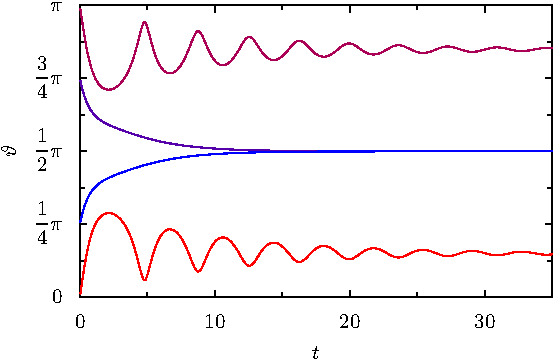
\includegraphics[scale=0.5]{theta.pdf}
    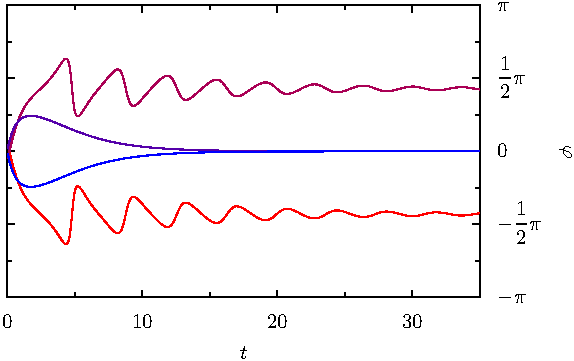
\includegraphics[scale=0.5]{phi.pdf}
    \end{center}
}

\section{nicht-autonome, nicht-lineare Differentialgleichungen}
\subsection{Motivation}
\frame {
    \frametitle{Kurze Zusammenfassung}

    \begin{enumerate}
    \item Umschreiben der DGL als System 1. Ordnung
    \item Suchen von stationären Punkten
    \item Untersuchen der Stabilität der stationären Punkte
    \end{enumerate}

    \only<2>
    {
    \vfill
    \begin{center}
    \Large Was bei nicht-autonomen Systemen?
    \end{center}
    }
}

\subsection{Beispiel}
\frame {
    \frametitle{Nicht-autonome Systeme}

    Differentialgleichung:
    \begin{equation}
    \nonumber
    \left(\begin{array}{c} \dot\vartheta \\ \dot\varphi\end{array}\right) =
    \left(\begin{array}{c}
    A\sin\varphi+C\cos\varphi\cos\vartheta \\
    A \frac{\cos\vartheta}{\sin\vartheta}\cos\varphi + B\cos\vartheta - C\frac{\sin\varphi}{\sin\vartheta} - \mu_0 + \mu_1\sin{(\omega t)}
    \end{array}\right)
    \end{equation}

    \pause
    \vfill

    Untersuchung:
    \begin{itemize}
    \item stroboskop-artige Popagation:

    \begin{equation}
    \nonumber
    \left(\begin{array}{c}
    \vartheta(nT) \\ \varphi(nT)
    \end{array}\right), \quad T=\frac{2\pi}{\omega}, \quad n\in\mathbbm{N}
    \end{equation}
    \item Bifurkationsdiagramm
    \item Attraktor
    \end{itemize}
}

\subsection{Bifurkationsdiagramm}
\frame {
    \frametitle{Bifurkationsdiagramm}

    \begin{center}
    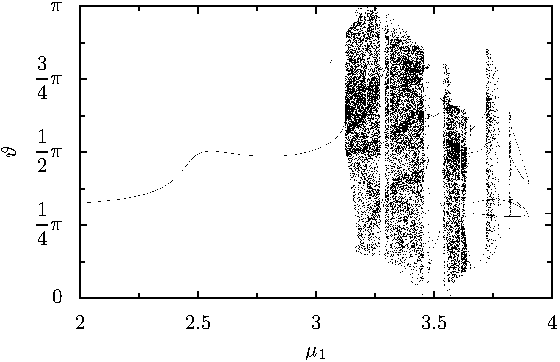
\includegraphics[scale=1.1]{bifurc_mu1.pdf}

    Parameter: $A=2$, $B=1$, $C=0.4$, $\mu_0=1$, $\omega=1$
    \end{center}
}

\subsection{Seltsamer Attraktor}
\frame {
    \frametitle{Seltsamer Attraktor}

    \begin{center}
    \only<1> { 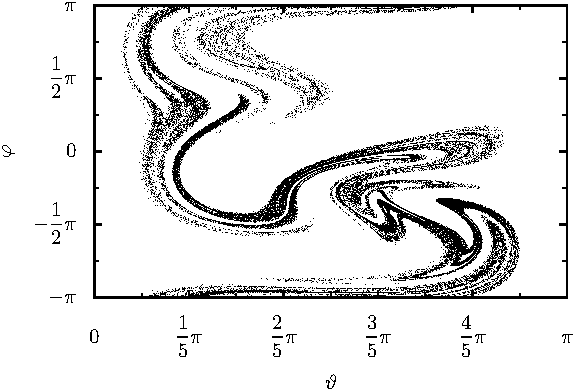
\includegraphics[scale=1.1]{strangeattractor.pdf} }
    \only<2> { 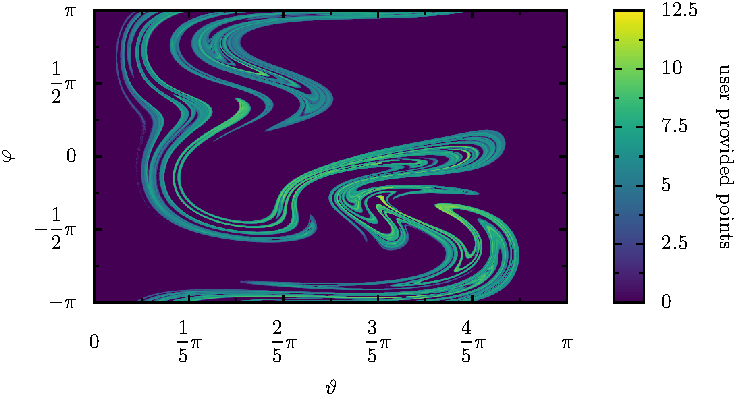
\includegraphics[scale=1.04]{density.pdf} }

    Parameter: $A=2$, $B=1$, $C=0.4$, $\mu_0=1$, $\mu_1=3.4$, $\omega=1$
    \end{center}
}

\frame {

    \begin{center}
    \huge Vielen Dank für die Aufmerksamkeit!
    \end{center}
}


\end{document}
